Un diagramma di fase (o diagramma di stato) è un particolare diagramma cartesiano sperimentale riferito ad una sostanza pura o ad una miscela, che rappresenta lo stato del sistema termodinamico in esame al variare di due o più coordinate termodinamiche (temperatura, pressione, volume, composizione chimica (frazione molare)).

\subsection{Diagramma di fase per singole speci chimiche}

\begin{figure}[H]
    \centering
    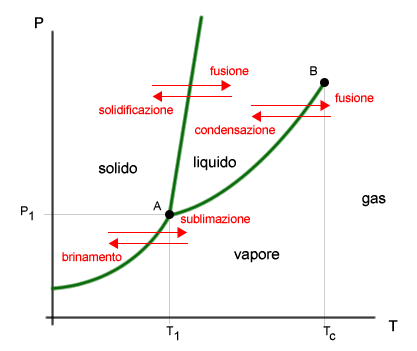
\includegraphics[width=8cm]{immagini/diagramma_di_stato.png}
\end{figure}

Tale grafico è inerente ad una singola specie chimica. Esso ha la temperatura sulle ascisse e la pressione sulle ordinate. Siccome non riguarda una soluzione non avremo una frazione molare. In esso troviamo le fasi e la loro esistenza, cioè le \textbf{regioni di esistenza} (che corrispondono a coppie di valori di temperatura e pressione) che permettono l'esistenza di tale fase.

Lungo le linee abbiamo coesistenza di due fasi. Laddove sono presenti più di una fase insieme si parla di equilibrio eterogeneo, il quale resta in equilibrio quando non varia il numero di fasi coesistenti in esso.

Il punto di intersezione delle linee di coesistenza è detto \textbf{punto triplo}, in cui si ha la coesistenza di tutte e tre le fasi.

In che modo possiamo muoverci lungo tale diagramma (il che corrisponde a variare pressione e temperatura), pur mantenendo lo stesso stato di partenza?

\begin{itemize}
    \item Se ci troviamo in una delle cosiddette regioni di esistenza, ad esempio quella dello stato solido, possiamo variare indipendentemente pressione e temperatura entro un certo limite restando nel medesimo stato. Poiché le due variabili sono indipendenti, si dice che tali regioni sono \textit{bi-varianti};
    \item Se invece ci troviamo sulle linee non possiamo variare pressione e temperatura indipendentemente l'una dall'altra: la variazione di una delle due determinerà automaticamente la variazione dell'altra, altrimenti la coesistenza di due fasi non verrà preservata. Quindi lungo le linee una delle due variabili è indipendente mentre l'altra è dipendente, per cui esse sono dette \textit{mono-varianti};
    \item Se infine ci troviamo sul punto triplo non possiamo variare né la pressione né la temperatura, altrimenti perderemmo la coesistenza dei tre stati e quindi l'equilibrio eterogeneo. Per questo motivo esso è detto \textit{zero-variante}.
\end{itemize}

\subsubsection{Diagramma di stato dell'acqua}
Consideriamo il diagramma di stato dell'acqua:

\begin{figure}[H]
    \centering
    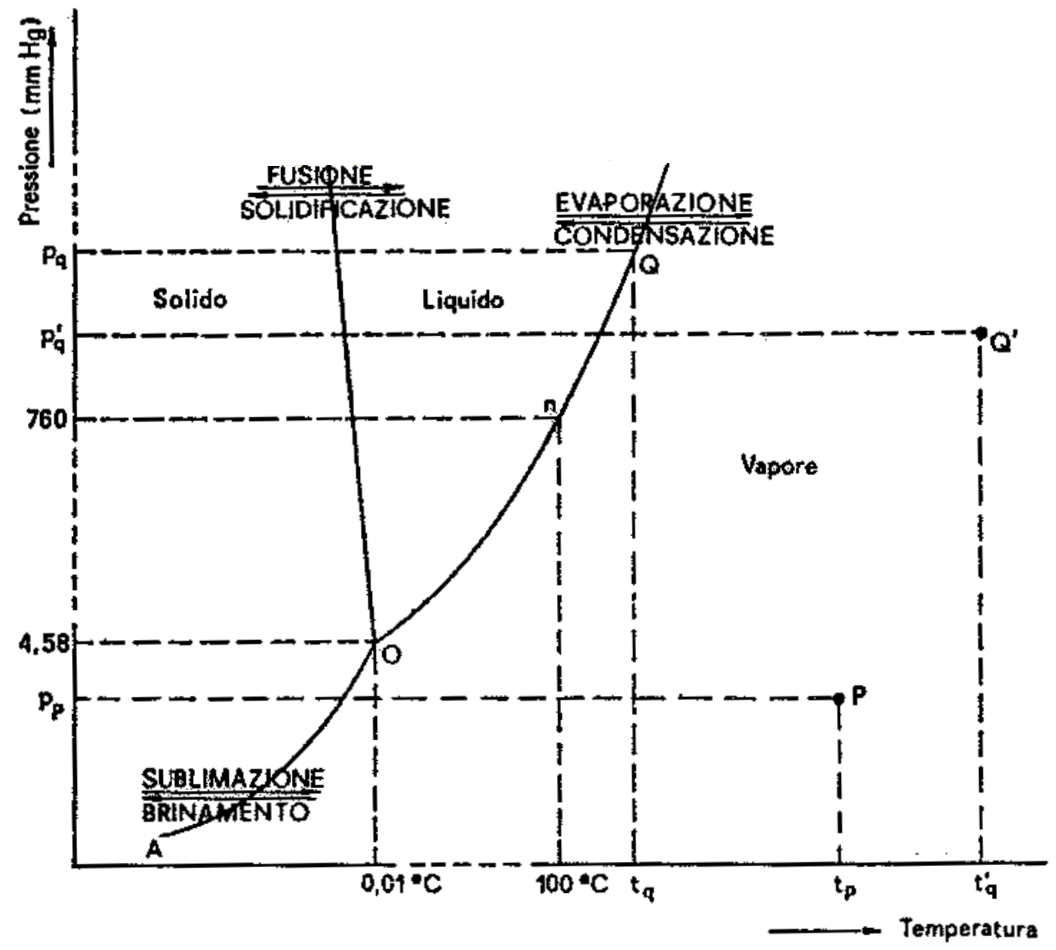
\includegraphics[width=10cm]{immagini/diagramma_di_stato_acqua.png}
\end{figure}

Abbiamo detto che esso è un diagramma sperimentale. Come si fanno le misure?

Immaginiamo di avere un cilindro munito di pistone in cui è preventivamente fatto il vuoto e dentro di esso mettiamo dell'acqua. Il sistema è tale da permetterci di misurare la temperatura interna e la tensione di vapore.

Per realizzare il diagramma si realizzano due esperimenti diversi. In un primo esperimento variamo la temperatura (si parte da basse temperature) e andiamo a misurare la tensione di vapore dell'acqua corrispondente. Partendo da temperature basse (-60° C) fino ad arrivare a 0°C (punto in cui iniziamo ad avere acqua) riusciamo a tracciare la linea in basso a sinistra. In queste condizioni il ghiaccio passerà allo stato di vapore, per cui stiamo studiando l'equilibrio ghiaccio vapore. Aumentando ancora la temperatura (arrivando fino a 374.1° C che è la temperatura critica) tracciamo la linea di destra. In questo caso studieremo l'equilibrio liquido-vapore.

Nel secondo esperimento invece variamo la pressione attraverso il pistone e andiamo a misurare la temperatura di fusione del ghiaccio corrispondente. In questo modo tracciamo la linea in alto, in quanto studiamo l'equilibrio liquido-solido. In particolare ci si accorge che man mano che aumentiamo la pressione (partiamo da 1 atm e arriviamo anche fino a 2030 atm) il ghiaccio fonde a temperature via via più basse.

Riportando le misure su un grafico otteniamo il diagramma di sopra.

L'acqua è l'unica sostanza che, al diminuire della temperatura, aumenta in volume. Ciò nel diagramma si traduce con una pendenza negativa della linea che separa solido e liquido. Tutti gli altri diagrammi infatti hanno tale linea con pendenza positiva.

Nei fatti a circa 4° C l'acqua ha la sua massima densità. Il motivo è che quando l'acqua viene raffreddata vengono favoriti i legami a idrogeno. Si realizza quindi un sistema esteso di interazioni e per mantenerle l'acqua aumenta di volume.

Il punto triplo dell'acqua si ha a 0.01° C, temperatura alla quale l'acqua esercita una tensione di vapore di 4.58 torr. In queste condizioni si ha coesistenza di acqua solida, liquida e vaporea.
\subsubsection{Diagramma di stato per CO$_2$}

Vediamo ora un esempio in cui il confine di fase tra solido e liquido ha pendenza positiva: il diagramma di stato dell'anidride carbonica. Esso si ottiene con lo stesso metodo sperimentale sopra descritto.

\begin{figure}[htp]
    \centering
    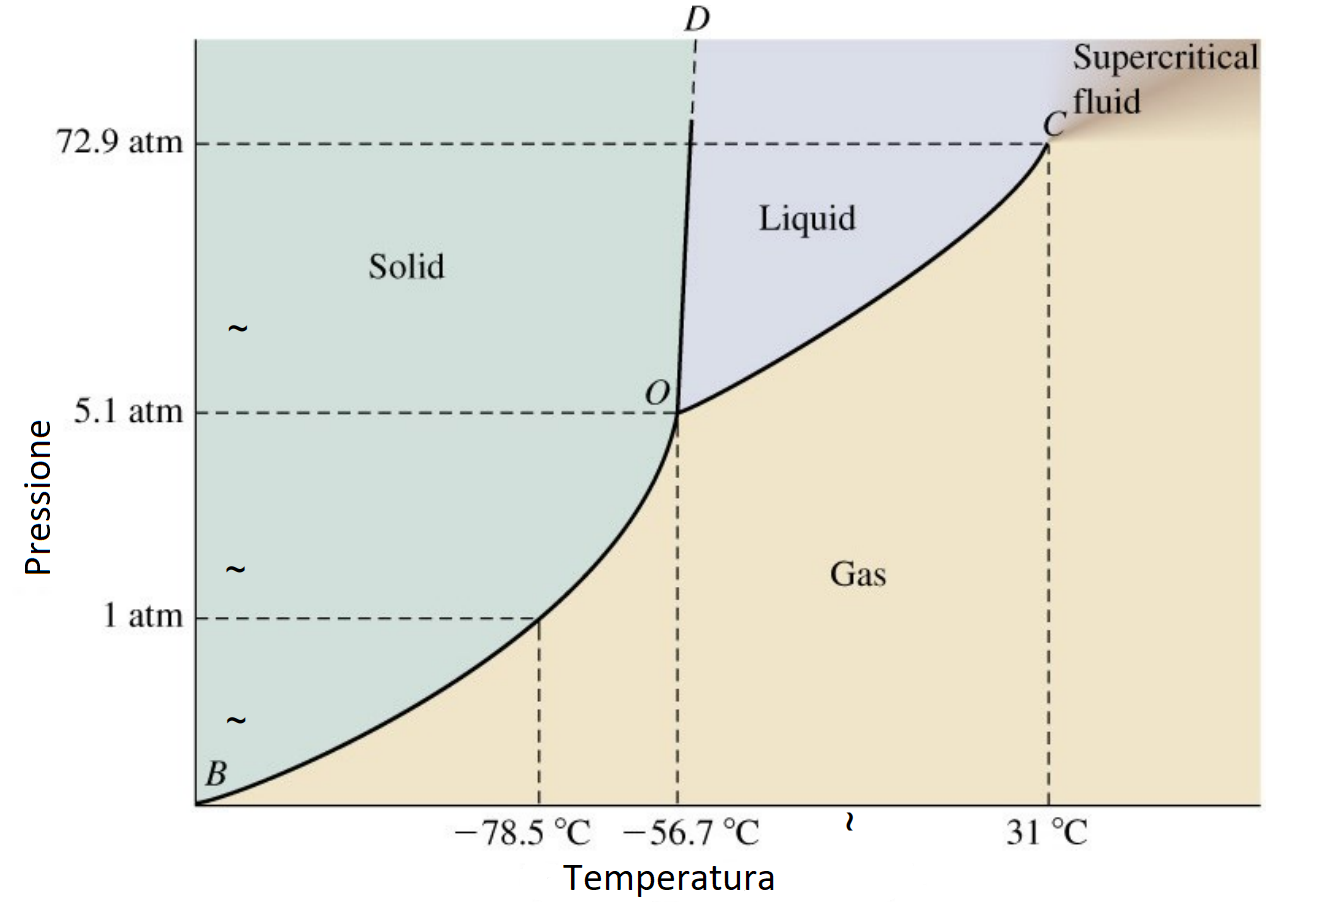
\includegraphics[width=12cm]{immagini/diagramma_di_stato_CO2.png}
\end{figure}

L'anidride carbonica solidifica facilmente, e infatti si ha una pendenza ripida, stavolta però sarà positiva.

Il punto triplo si trova a -56.7° C e 5.1 atm.

\subsection{Diagramma di fase per soluzioni}
\subsubsection{Diagramma di fase della granita}

\begin{figure}[htp]
    \centering
    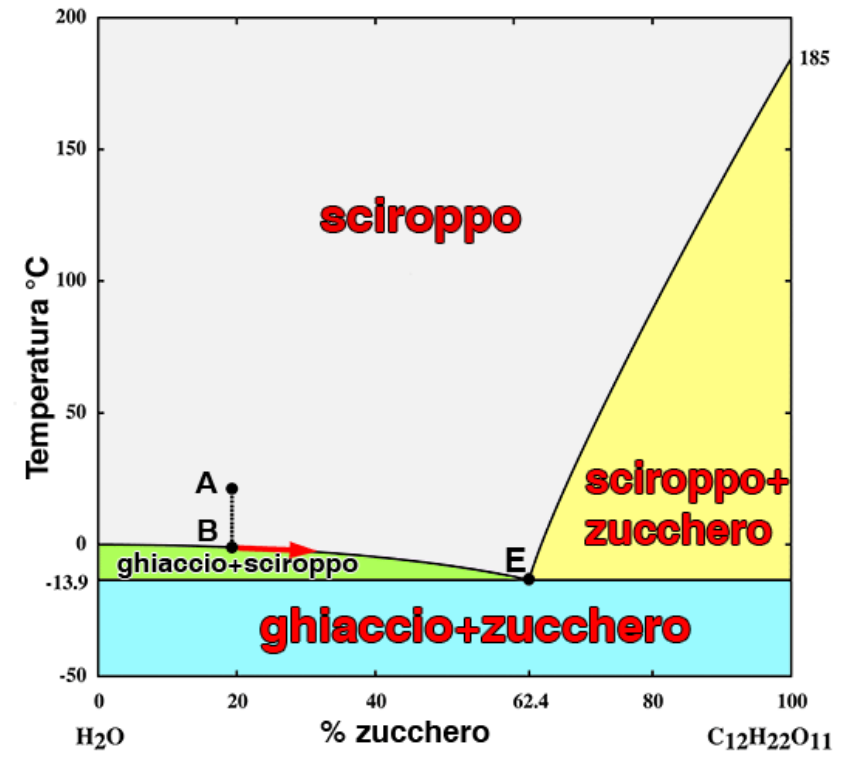
\includegraphics[width=10cm]{immagini/diagramma_di_stato_sciroppo.png}
\end{figure}

Avendo due componenti ricompare la frazione molare, perché possiamo avere infinite soluzioni al variare della composizione, quindi avremo la percentuale dei componenti in ascisse e la temperatura in ordinate.

Immaginiamo di avere una soluzione di acqua e il 20\% di zucchero (saccarosio) in massa.

Partiamo dal punto A che mostra questa composizione alla temperatura di 20° C. Raffreddiamo lentamente, in modo da avere una successione di stati di equilibrio, fino a raggiungere gli 0° C. Se fosse stata acqua pura avremmo già del ghiaccio, ma non essendola questo non si forma. Abbassando ulteriormente la temperatura iniziano a formarsi i primi cristalli di ghiaccio (non di soluzione ghiacciata!), cioè si sta separando un po' di solvente che diventa solido.

Dato che stiamo togliendo solvente, la soluzione si sta concentrando, per cui per poter continuare ad avere la solidificazione dobbiamo continuare ad abbassare la temperatura, perché a una soluzione pià concentrata corrisponde una temperatura di congelamento più bassa.

La concentrazione aumenta e il punto di congelamento diminuisce fino al raggiungimento del punto E, che è detto \textbf{punto eutettico}: in tale punto la composizione del solido che si forma è uguale a quella della soluzione da cui si separa. Tale composizione è detta \textit{eutettica} e arrivati a questo punto si inizia a formare il primo cristallo solido di soluzione, ossia iniziano a ghiacciare insieme acqua e zucchero.

In questo caso particolare abbiamo una temperatura eutettica di -13.9° C e una composizione eutettica fatta al 62.4\% di zucchero. Per temperature più basse di quella eutettica troviamo la soluzione che ghiaccia, cioè ghiaccio e zucchero insieme come solido.

Prima del punto eutettico e sopra la temperatura eutettica troveremo ghiaccio e sciroppo, cioè ghiaccio più acqua e zucchero liquidi insieme.

Se invece la concentrazione iniziale è più a destra di quella eutettica, avremo sciroppo più zucchero. Ciò significa che abbiamo usato così tanto zucchero che non si è sciolto, pertanto avremo una parte liquida formata da acqua e zucchero sciolto più una parte solida formata dallo zucchero che non si è sciolto e che è detto \textit{corpo di fondo}, cioè la parte di zucchero che non è solubilizzata e va a fondo de recipiente. In questo caso allora si parla di \textbf{soluzione satura}, cioè una soluzione che ha sciolto la quantità massima di soluto possibile.

Le regioni di esistenza allora sono:

\begin{itemize}
    \item Sciroppo: acqua + zucchero liquidi;
    \item Sciroppo più zucchero: acqua + zucchero liquidi e zucchero solido, non sciolto;
    \item Ghiaccio più zucchero: ghiaccio + zucchero solidi insieme;
    \item Ghiaccio più sciroppo: ghiaccio solido puro e acqua + zucchero liquidi.
\end{itemize}

Questo diagramma ci permette di capire quali condizioni attuare per avere una certa composizione della soluzione.
\subsubsection{Diagramma di fase della salamoia}

\begin{figure}[htp]
    \centering
    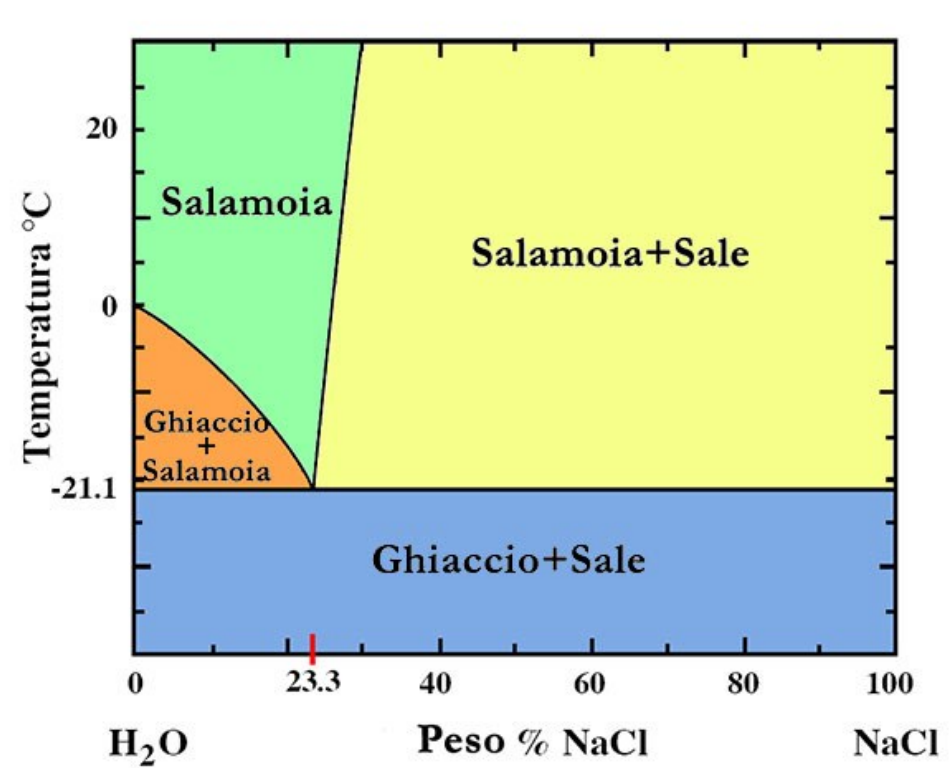
\includegraphics[width=10cm]{immagini/diagramma_di_stato_salamoia.png}
\end{figure}

La salamoia è una soluzione di acqua e sale.

Le regioni di esistenza sono:

\begin{itemize}
    \item Salamoia: acqua + sale liquidi (qui ci teniamo gli alimenti);
    \item Ghiaccio più salamoia: acqua + sale liquidi e ghiaccio puro. Si ottiene abbassando la temperatura.
    \item Salamoia più sale: acqua + sale liquidi e sale solido. Trovarsi in questa regione significa aver esagerato col sale, per cui nell'acqua che avevamo a disposizione non si riesce a sciogliere tutto il sale. Pertanto la soluzione avrà un corpo di fondo, formato dal sale solido.
    \item Ghiaccio più sale: ghiaccio + sale solidi insieme
\end{itemize}

La composizione eutettica per la salamoia viene raggiunta a -21.1° C con una concentrazione del 23.3\% di NaCl. Abbassando ulteriormente la temperatura inizieremo ad avere il solido composto da ghiaccio e sale.